\apendice{Especificación de diseño}

\section{Introducción}
En este apartado se van a explicar elementos del diseño del proyecto que explican su funcionamiento y estructura.

\section{Plantilla base de la que se ha partido}
Antes de nada es necesario mencionar que este trabajo ha partido de una platilla que ofrece Unity como punto de partida. Esa plantilla se llama Platformer Microgame y se puede añadir a la lista de assets en el siguiente enlace:\\
 \url{https://bit.ly/3wZEU8W}.\\ 
De esta plantilla se ha conservado sobre todo los elementos estéticos, pero también se ha conservado la clase Simulation y los eventos que esta lanza.

\subsection{Clase Simulation}
La calse Simulation es una clase encargada de manejar los eventos del juego. El objeto GameController hace uso de esta clase para ir ejecutando los eventos a medida que entran en cola. Esta clase tiene una particularidad de C\#. Simulaion es una “partial class”. Esto permite que la clase Simulation se construya en varios ficheros distintos. Para el funcionamiento de la clase Simulation, esta hace uso de otras dos subclases: Simulation.Event y Simulation.InstanceRegister. Se va a explicar a continuación por qué son clases que se consideran importantes y claves para entender el funcionamiento de la arquitectura del videojuego.

\textbf{Simulation:} Este fichero contiene la estructura principal del funcionamiento de Simulation. Simulation es una clase estática con una cola, también estática, que guarda eventos (clase Event) y los libera cuando GameController llama al método tick(). Este fichero tiene el método tick() y los métodos necesarios para añadir y remover elementos de la cola. 

\textbf{Simulation.Event:} Contiene la clase interna Event que se encarga de ejecutar el comando asociado a ese evento. De esta clase de la que heredan todos los eventos que saltan durante la ejecución del juego (como por ejemplo EnemyDeath, el evento que salta cuando el jugador muere). Los eventos se guardan en su mayoría en la carpeta Assets/Scripts/Gameplay.

\textbf{Simulation.InstanceRegister:} Contiene la clase InstanceRegister. Esta clase simplemente devuelve una instancia nueva de un objeto cualquiera. Esta clase está creada para que Simulation pueda crear singletons (patrón de diseño) de clases. Es utilizado para que todas las clases trabajen sobre el mismo modelo. Ese modelo es un script denominado PlataformerModel con una clase que exclusivamente tiene una serie de atributos (como el Player, las cámaras o el punto de aparición del jugador) que serán utilizados por varias clases.

\subsection{Eventos}
Los eventos son toda las clases que heredan de Simulation.Event. Todos los eventos se encuentran en la carpeta Assets/Scripts/Gameplay. Casi todas las clases evento del proyecto se han mantenido intactas de Platformer Microgame, sin embargo algunas eventos han sido modificados y otros añadidos.\\
Eventos modificados:
\begin{itemize}
\item
DisablePlayerInput.
\item
EnablePlayerInput.
\item
PlayerDeath.
\item
PlayerEnteredVictoryZone.
\end{itemize}

Eventos añadidos:
\begin{itemize}
\item
SetGameInitialState: Evento que se lanza para forzar volver la escena al estado inicial.
\item
PlayerObstacleCollision: Evento que salta cuando el Player colisiona con un obstáculo. Este evento mata al jugador.
\item
LoadGameMenu: Evento que carga la escena del menú principal y cambia a ella.
\end{itemize}

\section{Diseño de datos}
Los datos necesarios para el desarrollo de un videojuego son los Sprites y los audios utilizados durante su ejecución.

Para utilizar estos recursos en Unity se hace uso de los AudioSources \cite{AudioSource} y los SpriteRenderers \cite{SpriteRenderer}.

\subsection{AudioSource}
La clase AudioSource es la clase de la que hace uso Unity para reproducir audios. Esta clase tiene un atributo público AudioClip que contendrá el audio que se va a reproducir. Se puede saber si el audio se está reproduciendo con el atributo booleano isPlaying.\\
Se puede modificar el volumen de reproducción de todo audio reproducido con ese AudioSource.

Los métodos de reproducción de audios son los siguientes:
\begin{itemize}
\item
Play: reproduce el audio asociado al AudioSource (AudioSource.AudioClip).
\item
PlayDelayed: reproduce el audio asociado al AudioSource despues del tiempo pasado por parámetros.
\item
PlayOneShot: permite reproducir cualquier audio pasado como parámetro. El audio que se desea reproducir deberá estar encapsulado en una instancia de la clase AudioClip \cite{AudioClip}.
\end{itemize}

En el proyecto desarrollado AudioSource se ha usado para controlar el volumen del juego. Se ha creado una clase VolumeManager encargada de guardar y modificar el volumen general del juego y el volumen de la música.\\
Sin embargo, los AudioSources del juego están protegidos por clases envoltorio encargadas de modificar el volumen del juego de acuerdo a las opciones de juego.

\begin{figure}[h]
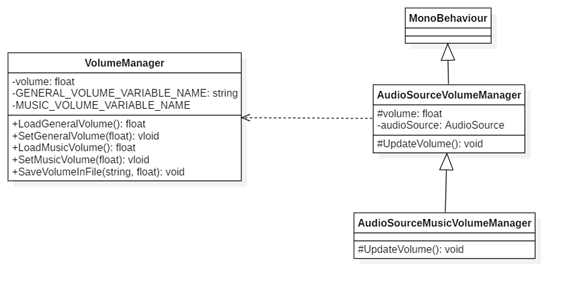
\includegraphics[scale=1]{Memoria/Aspectos_relevantes/Volumen_persistente/VolumeManager_UML}
\caption{Diagrama UML de las clases que hacen uso del AudioSource}
\end{figure}

\subsection{SpriteRenderer}
La clase SpriteRenderer es la encargada de hacer que se muestre una imagen en una zona del videojuego. Para poder mostrar las imágenes en Unity hay que utilizar la clase envoltorio Sprite. SpriteRenderer tiene un atributo público Sprite que contiene la imagen que mostrará ese SpriteRenderer.

En el proyecto se ha hecho uso de esta clase para mostrar imágenes estáticas y para mostrar animaciones.\\
Para crear las animaciones se ha creado dos clases SpriteAnimator y OneTimeAnimator. Estas clases simulan la animación intercalando a grandes velocidades un conjunto de imágenes. La diferencia entre estas dos clases es que SpriteAnimator reproduce una animación indefinidamente en bucle y OneTimeAnimator reproduce la animación una sola vez.

\begin{figure}[h]
\centering
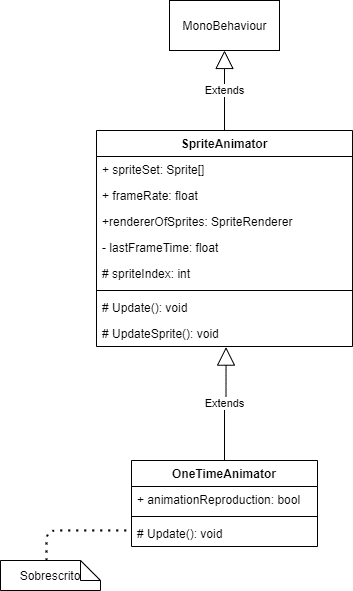
\includegraphics[scale=0.8]{Memoria/Aspectos_relevantes/Animadores/Herencia_animators}
\caption{Diagrama UML de las clases SpriteAnimator y OneTimeAnimator}
\end{figure}

\section{Diseño procedimental}
En este apartado se explicarán los algoritmos que se han desarrollado para el correcto funcionamiento del videojuego.

\subsection{Sistema de colisiones}
Para simular el sistema de colisiones se optó por utilizar la velocidad como elemento principal.

\clearpage
\begin{figure}[h]
\centering
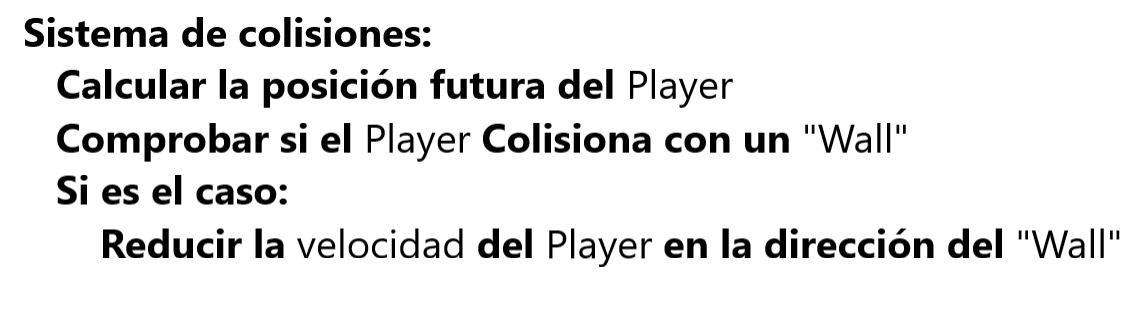
\includegraphics[scale=0.55]{Anexos/Anexo_C/Pseudocodigo_colisiones}
\caption{Pseudocódigo que resume el sistema de colisiones}
\end{figure}

Para saber si un KinematicObject va a colisionar con el suelo o un muro (se identifican los objetos con los que se desea chocar porque tienen asignada la layer “Wall”) se coge la velocidad del KinematicObject (se obtiene del atributo velocity del Rigidbody2D), que está representada en unidades/segundo. Con la velocidad que lleva el KinematicObject y su posición se puede deducir la siguiente posición en la que se encontrará.

Hay un método que se llama Physics2D.BoxCast con el que se puede crear un rectángulo en una región del espacio y comprobar si se colisiona con algún objeto. En caso de colisionar con un objeto se devuelve un objeto de la clase RayCastHit2D con toda la información relativa a la colisión. Hay un método similar a Physics2D.BoxCast que es Physics2D.BoxCastAll que hace lo mismo, pero devolviendo un vector de RayCastHit2D con un elemento por cada objeto con el que has colisionado.

Se puede filtrar las colisiones por Layer, pudiendo solo tener en cuenta las colisiones con objetos que tengan asociada una Layer con el mismo nombre que el pasado por parámetro en el método. Para el sistema de colisiones solo se han tenido en cuenta los objetos con Layer igual a “Wall”.

Con el método Physics2D.BoxCastAll se va a crear un rectángulo del tamaño del Collider2D del KinematicObject en la siguiente posición en la que se encontrará el objeto y comprobarán cuántos objetos con Layer igual a “Wall” colisionarán en esa posición con el KinematicObject.

\clearpage
\begin{figure}[h]
\centering
\includegraphics[scale=1]{Memoria/Aspectos_relevantes/Sistema_Colisiones/Detección_colisiones}
\caption{Simulación del proceso de detección de colisiones}
\end{figure}

Una vez detectados con que muros se han colisionado (objetos con Layer igual a “Wall”) se va a simular el choque modificando la velocidad del KinematicObject poniendo a cero la velocidad en la dirección de la colisión del muro. Un ejemplo de aplicación sería un KinematicObject yendo a una velocidad marcada por el vector (1, -2), es decir 1 unidad hacia la derecha (eje x) y dos unidades hacia abajo (eje y). Si se detecta que se va a colisionar contra el suelo (un muro que está a los pies del KinematicObject) la velocidad debería establecerse al vector (1,0), es decir continuar el desplazamiento a la derecha pero cesar el movimiento hacia abajo.

Para calcular en qué dirección hay que limitar la velocidad se utiliza el vector normal de la recta creada por la pared más cercana del muro. Ese vector normal lo ofrece el objeto RayCastHit2D en su atributo “normal”.
Se va a añadir una figura explicativa:

\clearpage
\begin{figure}[h]
\centering
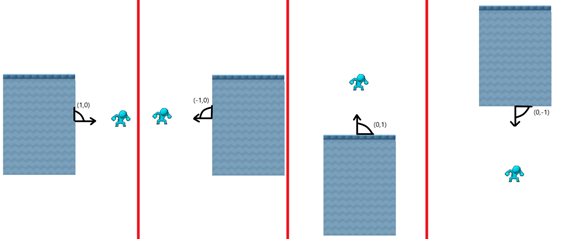
\includegraphics[scale=1]{Memoria/Aspectos_relevantes/Sistema_Colisiones/Vector_normal}
\caption{Vector normal del muro en función de la posición del KinematicObject}
\end{figure}

De la colisión del KinematicObject se encarga el objeto KinematicObjectCollisionManager, que tiene una referencia a KinematicObject y se encarga de llamar al método Physics2D.BoxCastAll y limitar la velocidad del KinematicObject en caso de colisión.

\begin{figure}[h]
\centering
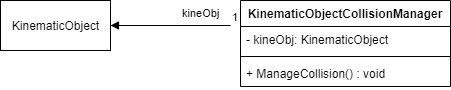
\includegraphics[scale=1]{Memoria/Aspectos_relevantes/Sistema_Colisiones/KinematicObjectCollisionManager_UML}
\caption{Diagrama UML del sistema de colisiones}
\end{figure}

\subsection{Modificaciones gravitatorias}
Durante la ejecución del juego puede ser que los objetos kinemáticos sufran modificaciones que varíen las fuerzas gravitatorias que los afectan. Estas modificaciones las provocan los modificadores de gravedad y no afectan a todos los elementos del juego sino a un objeto kinemático en concreto.

Dada esta premisa, se ha creado una clase KinematicObjectGravityManager encargada de la gestión de las modificaciones de gravedad que afectan al KinematicObject.

\begin{figure}[h]
\centering
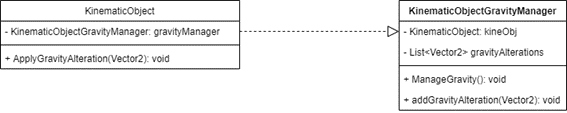
\includegraphics[scale=0.6]{Memoria/Aspectos_relevantes/Modificaciones_gravitatorias/KinematicObjectGravityManager_UML}
\caption{Diagrama UML de la clase encargada de la gestión de la gravedad del KinematicObject}
\end{figure}

KinematicObjectGravityManager va a funcionar mediante una lista a la que se van a ir añadiendo objetos de clase Vector2 que representarán las alteraciones de la gravedad. En cada llamada al método FixedUpdate de KinemticObject se recorre la toda la lista acumulando las alteraciones gravitatorias y se aplican esas alteraciones al efecto gravitatorio por defecto (Physics2D.gravity) y se simula la gravedad. Después de este proceso se vacía la lista.

\begin{figure}[h]
\centering
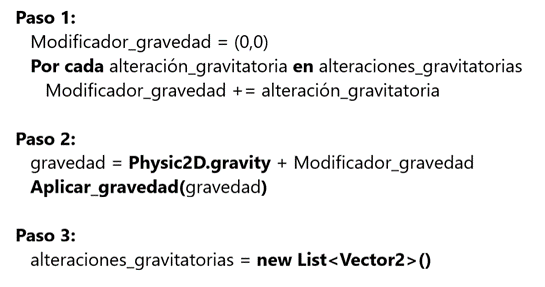
\includegraphics[scale=1]{Memoria/Aspectos_relevantes/Modificaciones_gravitatorias/Pseudocodigo_modificadores_gravedad}
\caption{Pseudocódigo del proceso de modificación de la gravedad del KinematicObject}
\end{figure}

Hay dos tipos de modificadores de gravedad: los obstáculos superdensos y los inversores de gravedad. La diferencia fundamental entre estos modificadores de gravedad es que los obstáculos superdensos aplican una modificación temporal mientras que los inversores de gravedad modifican la gravedad de forma permanente (o hasta que se cancele el efecto).

\subsection{TimeAffectedObjects}
Hay una serie de objetos que se ven afectados por las modificaciones temporales particulares. Estos objetos heredarán de la clase TimeAffectedObject. 

\begin{figure}[h]
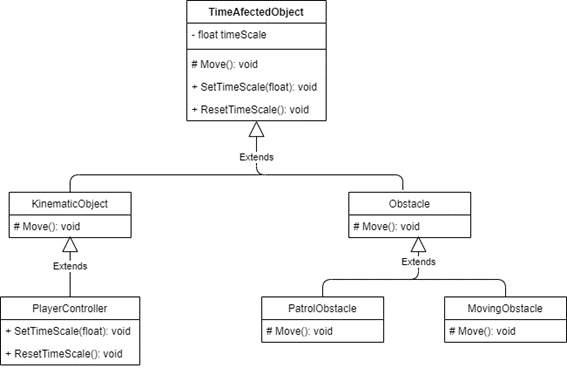
\includegraphics[scale=1]{Memoria/Aspectos_relevantes/Tiempo_bala/Herencia_TimeAffectedObject}
\caption{Clases que heredan de TimeAffectedObject}
\end{figure}

El movimiento de las clases que hereden de esta deberá implementarse en el método Move, pues será en ese método en el que se aplicará la modificación temporal al movimiento acelerándolo o ralentizándolo según toque.

Cuando el juego vuelva al estado inicial será necesario restablecer la escala temporal de todos los TimeAfectedObjects a la escala por defecto.

\begin{figure}[h]
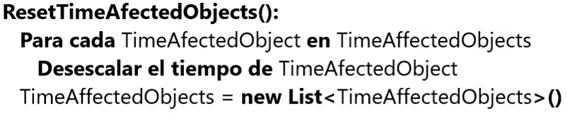
\includegraphics[scale=1]{Memoria/Aspectos_relevantes/Tiempo_bala/Pseudocodigo_TimeAffectedObject}
\caption{Pseudocódigo del método llamado para resetear los TimeAfectedObject}
\end{figure} 

\section{Diseño arquitectónico}
\subsection{GameController}
Durante la ejecución de las escenas hay elementos que se requiere que estén en una posición inicial y que se pueda volver a ella cuando se requiera (concretamente cuando el Player muera y se tenga que volver al estado inicial de la escena).\\
Los objetos que gestiona el GameController puede ser cualquier GameObject, pero no todos necesitarán ser reiniciados, pues tendrán un estado estable durante toda la ejecución de la escena. Por ejemplo, los obstáculos móviles se desplazan horizontal y pueden incluso ser destruidos, pero cuando el Player muera el obstáculo móvil tiene que volver a la posición inicial en la que se encontraba al cargar la escena. De esta labor se encargará el GameController. Sin embargo, el obstáculo inmóvil se mantiene siempre estático en la misma posición y no puede ser destruido, con lo que el GameController no tiene que preocuparse por devolverlo a un estado estable, pues es el único estado en el que puede estar.

\begin{figure}[h]
\centering
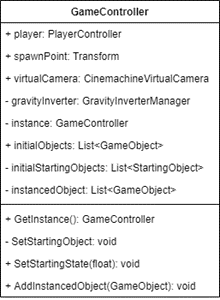
\includegraphics[scale=1]{Memoria/Aspectos_relevantes/GameController/GameController}
\caption{Diseño de la clase GameController}
\end{figure}

GameController está implementado de manera que simule el patrón de diseño Singleton, en la medida en la que Unity lo permite, llamándose en el método Awake al método GetInstance para asegurarse de que siempre se trabaja siempre sobre el mismo GameController, a pesar de que haya varias instancias de él.

\subsubsection{Funcionamiento del estado estable}
GameObject tiene tres atributos lista: initialObjects, initialStartingObjects e instancedObjects. De estas tres listas la única pública es initialObjects. La intención de esta lista es que se añada en el editor de Unity todos los elementos cuyo estado se desea que sean devueltos a un estado estable.\\
Cuando se llama al método Awake el contenido de initialObjects se vuelca en initialStartingObjects. InitialStartingObjects no es una lista de GameObject sino una lista de StartingObject. La clase StartingObject es una clase que contiene dos atributos: el GameObject que se desea poder devolver a un estado estable y un atributo Transform con la información necesaria para devolver el GameObject a la posición inicial.\\
Por último la lista instancedObject contiene los objetos que hay que se han devuelto al estado estable.

Estas tres listas pueden parecer redundantes, pero no lo son. Es cierto que entre intialObjects e initialStartingObjects no hay mucha diferencia, pero al ser pública la lista initialObjects se ha preferido crear una lista con un nivel de encapsulamiento privado y que haya tratado los elementos de initialObjects para adaptarse a la aplicación del estado estable. Los elementos de StartingObjects en realidad van a hacer la labor de prototipo. Esto se refiere a que los elementos de initialStartingObjects no van a aparecer en la escena, sino que van a ser utilizados para clonar GameObjects en el estado inicial deseado para que parezca que todos los elementos vuelven a su estado inicial, cuando en realidad están siendo destruidos e instanciados objetos iguales a los eliminados (esto es lo que hace el método SetStartingState).

Los elementos que tiene la lista instancedObjects son todos los GameObject que se van a destruir cuando se llame al método SetStartingState. InstancedObjects por supuesto tendrá todos los objetos clonados de initialStartingObjects, pero también contiene GameObjects que pueden ser creados en tiempo de ejecución, pero que al volver el juego a un estado inicial tienen que ser destruidos (como por ejemplo los obstáculos móviles que instancian las fábricas de obstáculos).

\begin{figure}[h]
\centering
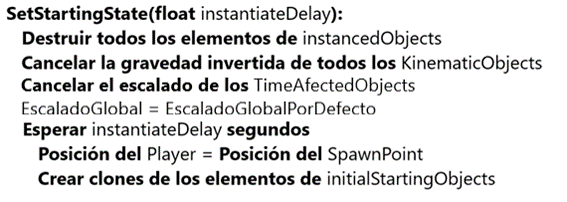
\includegraphics[scale=1]{Memoria/Aspectos_relevantes/GameController/Pseudocodigo_starting_objects}
\caption{Pseudocódigo que refleja todas las operaciones que hay que realizar para establecer un estado de juego inicial estable}
\end{figure}

\subsubsection{Clase PlatformerModel}
La clase PlatformerModel es una clase estática con atributos estáticos y sin métodos. La intención de esta clase es ofrecer acceso a una serie de objetos que pueden ser necesitados por cualquier clase en la escena. La única clase que debería asignar valores a PlatformerModel es GameObject, que lo hará exclusivamente en la llamada al método Awake y realizará la asignación una sola vez y no modificará en ningún momento más durante la ejecución los valores de los atributos de PlatformerModel. Los objetos que se podrán consultar mediante PlatformerModel son:
\begin{itemize}
\item
La CinemachineVirtualCamera que utiliza la escena (PlatformerModel.virtualCamera).
\item
El PlayerController asignado al avatar jugable (PlatformerModel.player).
\item
El objeto de tipo Transform asociado al punto de reaparición e inicio de escena del Player (PlatformerModel.spawnPoint).
\item
El GameController de la escena (PlatformerModel.gameController).
\item
El GravityInverterManager asociado a la escena \\ (PlatformerModel.gravityInverterManager).
\end{itemize}
Esta clase es muy útil para asegurar que todas las clases trabajan sobre los mismos objetos, sobre todo los eventos, pues puede resultar inadecuado hacer una cadena de mensajes para consultar los elementos principales de los niveles cada vez que sea necesario.

\subsubsection{Clase Simulation}
La clase Simulation está explicada más detalladamente en la sección de Trabajos relacionados. Pero a grandes rasgos la clase Simulation es una clase estática con una estructura de datos similar a una cola que alberga eventos y un método Tick. Ese método lo que hace es ir avanzando eventos en la cola y ejecutándolos hasta que la cola esté vacía o hasta que se encuentre un evento que debe ser ejecutado en un momento de la ejecución posterior al momento en el que se encuentra el programa.

\begin{figure}[h]
\centering
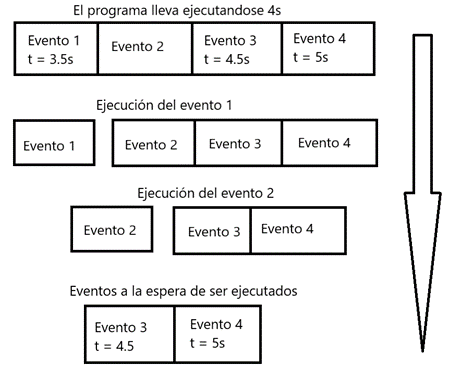
\includegraphics[scale=0.8]{Memoria/Aspectos_relevantes/GameController/Flujo_simulation}
\caption{Diagrama que representa un ejemplo de las operaciones llevadas a cabo en la llamada al método Tick}
\end{figure}
\clearpage

La clase GameController llama al método Tick de Simulation en cada llamada al Update.

\subsection{Estados del Player}
Los estados que utiliza PlayerController son una aplicación del patrón de diseño Estado que modificará el comportamiento del Player. Se ha tomado esta decisión porque las operaciones a realizar por PlayerController variarán en función de en qué situación se encuentre. Las situaciones en las que se encontrará el Player pueden cambiar en tiempo de ejecución y obligarán a realizar operaciones distintas.

A continuación se mostrará un diagrama con los posibles estados y las condiciones permiten pasar de uno a otro:

\clearpage
\begin{figure}[h]
\centering
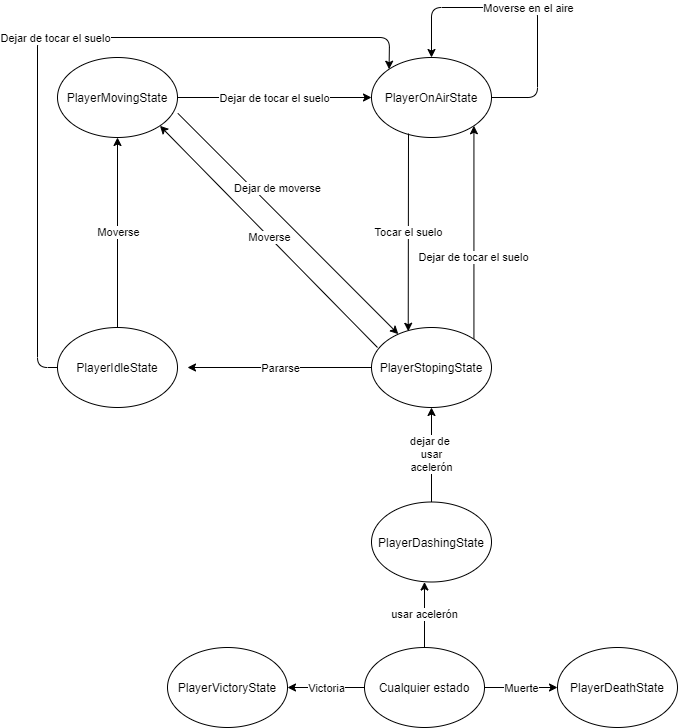
\includegraphics[scale=0.6]{Memoria/Aspectos_relevantes/Arquitectura_Player/Diagrama_de_estados}
\caption{Diagrama de transición entre estados de PlayerController}
\end{figure}

Todos los estados heredan de la interfaz PlayerState, que implementa los métodos UpdateState y FixedUpdateState. UpdateState será llamado en el método Update de PlayerController y FixedUpdateState será llamado por el método FixedUpdate de PlayerController. Los estados realizan las siguientes operaciones:
\begin{itemize}
\item
PlayerIdleState en realidad no realiza ninguna acción pues cuando el avatar está quieto no realiza ninguna acción, pero se encarga de pasar a otros estados cuando toque. De PlayerIdleState se puede pasar a PlayerMovingState si se pulsan los botones de movimiento. También se puede pasar a PlayerOnAirState si el Player no está en contacto con el suelo. De primeras puede parecer una transición innecesaria, pues estando quieto es improbable que se pase de estar tocando el suelo a no estar tocándolo. Esta transición principalmente se ha añadido porque PlayerIdleState es el estado por defecto. Se va a instanciar PlayerController con el estado PlayerIdleState y cada vez que se modifique el estado de PlayerController de manera externa a esta clase (por ejemplo cuando se reaparece después de morir) se asignará el estado PlayerIdleState a PlayerController. Añadiendo esa transición se asegura mantener un estado acorde con la situación para todos los casos, se asigne en el momento en el que se asigne el estado PlayerIdleState.
\item
PlayerOnAirState es el estado que se adoptará siempre que no se esté en contacto con el suelo (excepto cuando se esté realizando el acelerón). Este estado realiza una acción que es controlar el movimiento del Player en el aire, pues es ligeramente distinto al movimiento en el suelo. De este estado solo se puede pasar al estado PlayerStopingState cuando se toque el suelo.
\item
PlayerMovingState es el estado en el que se está cuando el Player se está moviendo por el suelo. Este estado se encarga de variar la velocidad del Player cuando se está moviendo en función de que botones de movimiento se están pulsando. Se puede pasar a los estados PlayerOnAirState, si al moverse el Player deja de estar en contacto con el suelo (caerse por un precipicio, por ejemplo) o al estado PlayerStopingState si el jugador deja de pulsar los botones de movimiento.
\item
PlayerStopingState se encarga de, cuando se cesa el movimiento, se realice una deceleración sobre el Player generando un efecto de parada orgánico. De este estado se puede volver al estado de PlayerMovingState si se vuelve a pulsar los botones de movimiento. A PlayerOnAirState se puede pasar si durante la deceleración se deja de tocar el suelo. Cuando se termine de decelerar y el Player se quede quieto se pasa al estado PlayerIdleState.
\item
PlayerDashingState es un estado un poco particular que no puede ser pisado por ningún otro. PlayerDashingState hace que el jugador valla a una velocidad constante durante un periodo de tiempo determinado sin verse afectado por las físicas como la gravedad. Aunque el Player no se vea afectado por las físicas durante el acelerón, las colisiones sí que se aplicarán sobre él. Cuando se termina de hacer el acelerón se pasa al estado PlayerStopingState.
\item
PlayerDeadState y PlayerVictoryState son dos estados cuya principal función es que el Player no realice ninguna función mientras se encuentren en ese estado. PlayerDeadState es un estado que se activa cuando el Player muere y se sale de él al hacer reaparecer al Player en la zona de reaparición, donde el Player pasará al estado PlayerIdleState. PlayerVictoryState es el estado final que alcanza el Player. Cuando se llega a la zona de victoria se pasa al estado PlayerVictoryState y no se sale de él, pues no hace falta. Cuando se llegue a la zona de victoria y se pase al PlayerVictoryState se pasará al siguiente nivel y por tanto no hará falta gestionar más los estados (los Player son independientes en cada nivel).
\end{itemize}

\begin{figure}[h]
\centering
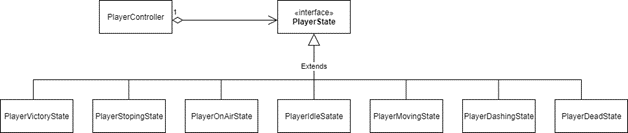
\includegraphics[scale=0.8]{Memoria/Aspectos_relevantes/Arquitectura_Player/Estados_Player}
\caption{Diagrama de herencia de los estados de PlayerController}
\end{figure}

Adicionalmente la interfaz PlayerState añade los métodos EnterPlayerState y ExitPlayerState donde los hijos implementan las instrucciones que es necesario hacer para que al entrar y salir del estado el Player se mantenga consistente, dando una implementación similar al patrón de diseño Método Plantilla.

\clearpage
Las instrucciones que se llevan a cabo cada vez que se cambia de estado son las siguientes:
\begin{figure}[h]
\centering
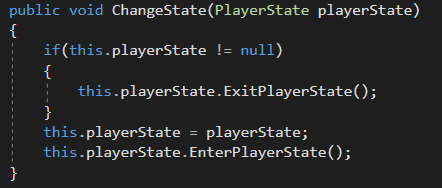
\includegraphics[scale=1]{Memoria/Aspectos_relevantes/Arquitectura_Player/Codigo_cambio_estado}
\caption{Código del Método Plantilla ChangeState}
\end{figure}

\subsection{Obstáculos que siguen una rutina y la clase PatrolPath}
Los obstáculos que siguen una rutina son obstáculos que viajan a través de una serie de puntos a una velocidad constante en un intervalo de tiempo marcado, de manera repetitiva hasta el final de la ejecución de la escena o el reinicio de esta. El punto de inicio y fin de la rutina coinciden. 

Realmente el obstáculo que sigue una rutina (PatrolObstacle) no calcula a donde tiene que moverse, sino que delega esta labor a la clase PatrolPath y mueve su posición a donde le indica el PatrolPath.

\begin{figure}[h]
\centering
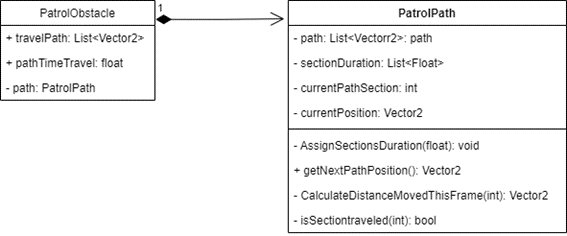
\includegraphics[scale=1]{Memoria/Aspectos_relevantes/Obstáculos/PatrolPath_UML}
\caption{Diagrama UML de la clase PatrolObstacle}
\end{figure}

PatrolPath recibe en el constructor la rutina que va a seguir el PatrolObstacle y el tiempo que tardará en recorrerla. PatrolPath calcula el tiempo que le llevará recorrer cada sección. Siendo que se tarda en hacer toda la rutina \textit{t} segundos, cada sección se tardará en recorrer $\dfrac{dy*d}{t}$

Siendo \textit{dy} la distancia euclidiana de la sección y \textit{d} la distancia total.

\begin{figure}[h]
\centering
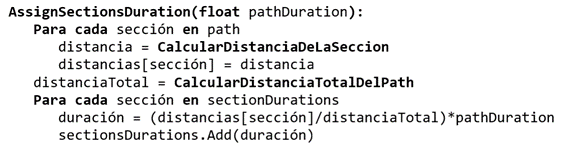
\includegraphics[scale=1]{Memoria/Aspectos_relevantes/Obstáculos/Pseudocodigo_asignar_duraciones}
\caption{Pseudocódigo de cálculo del tiempo que lleva recorrer cada sección}
\end{figure}

\clearpage
\begin{figure}[h]
\centering
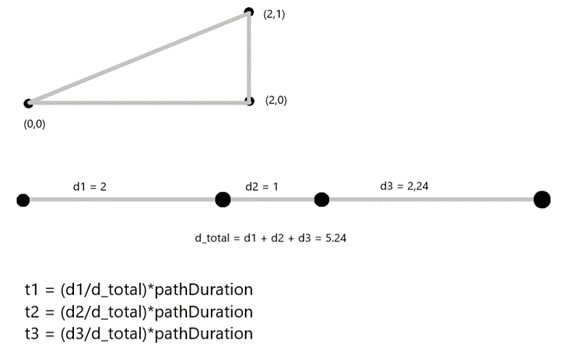
\includegraphics[scale=1]{Memoria/Aspectos_relevantes/Obstáculos/Diagrama_distancias_recorridas}
\caption{Cálculo del tiempo que se tarda en atravesar cada sección}
\end{figure}

PatrolPath sigue un diseño muy parecido al de un Iterador en el sentido de que el de la posición actual solo se puede obtener la siguiente y nada más.
La próxima posición del obstáculo que sigue una rutina (calculada en cada Update) se calcula sumando a la posición actual la distancia que se recorrerá cada frame (cada Time.deltaTime segundos).
La distancia que se recorre cada frame se puede obtener mediante la fórmula $\dfrac{(v1-v2)t}{ty}$

Siendo \textit{v1} el punto del que se parte, \textit{v2} el punto al que se quiere llegar, \textit{t} la fracción de espacio que se quiere recorrer (Time.deltaTime) en unidades de tiempo normalizado con\textit{ty} (el tiempo que se tarda en recorrer la sección) (en un frame se recorre un \textit{t/ty} sobre 1 de la distancia a recorrer).

\clearpage
\begin{figure}[h]
\centering
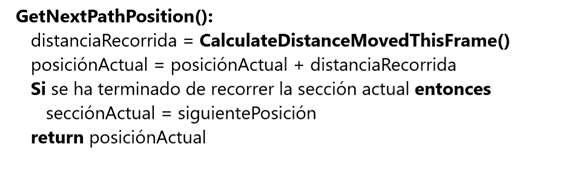
\includegraphics[scale=1]{Memoria/Aspectos_relevantes/Obstáculos/Pseudocodigo_siguiente_posicion}
\caption{Calcular la siguiente posición a la que debe moverse el obstáculo que sigue una rutina}
\end{figure}